\documentclass[12pt,a4paper]{article}
\usepackage[utf8]{inputenc}
\usepackage[english]{babel}
\usepackage{enumerate}
\usepackage{amsmath}
\usepackage{amsfonts}
\usepackage{amssymb}
\usepackage{graphicx}
\usepackage{fourier}
\usepackage[left=2cm,right=2cm,top=2cm,bottom=2cm]{geometry}
\usepackage{commath}
\usepackage{cancel}
\usepackage{placeins}
\author{Juan Carlos Apitz, ID 012523821}
\title{STAT572 - Homework Assignment 6}
\begin{document}

\maketitle

\section*{In-class - Density Estimation with Normal and Epan Kernels:}

\textbf{Part a.}\\

\textbf{Results \& Discussion: }
In this part of the problem we use the kernel method of density estimation applied to the random variable generated by $X_1,X_2,...,X_n \sim exp(\lambda=5)$. We use both the Normal and the Epanchnikov kernels and compare the results of generating 100 Monte Carlo simulations of the density estimates and corresponding mean squared errors (MSE) when $X_i = 5$.\\

The results below show that the approximations are fairly close to the actual values of the $exp(\lambda=5)$ pdf for $X = 5$. The MSE of the Normal kernel estimation is $5.809501\times10^{-6}$, and the MSE of the Epanchnikov kernel is $761647e\times10^{-6}$. Essentially zero. Figure \ref{inclass fig1} below shows the graphical representation which supports the close fit of the estimates as indicated by the MSE values.

\begin{figure}[ht!] 
\begin{center}
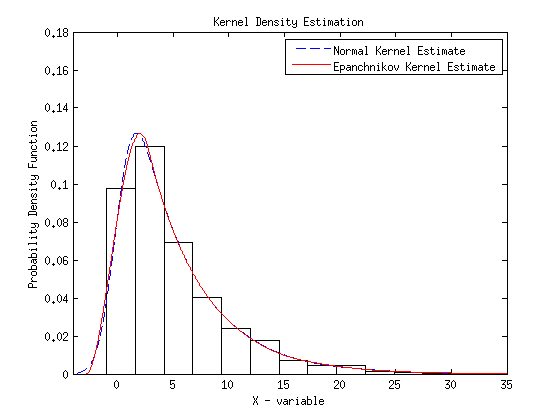
\includegraphics[scale=.87]{inclass_grapha.png}
\caption{Kernel Density Estimation of the Exponential pdf, $\lambda=5$.}
\label{inclass fig1}
\end{center}
\end{figure}
\FloatBarrier
\clearpage
\textbf{MSE Results}
\begin{verbatim}
>> density_est

MSE using Normal Kernel density estimation: 5.809501e-06

MSE using Epan Kernel density estimation: 9.761647e-06
\end{verbatim}

\textbf{Code}
\begin{verbatim}
% Take rs of size 100 from exp(5)
n = 1000;
data = exprnd(5,1,n);

% Use Normal Reference Rule for bin width
% of frequency histogram.
h = 2.15*sqrt(var(data))*n^(-1/5);
t0 = min(data)-1;
tm = max(data)+1;
bins = t0:h:tm;
vk = histc(data,bins);
vk(end) = [];
fhat = vk/(n*h);
bc = (t0+h/2):h:(tm-h/2);
bar(bc,fhat,1,'w')
hold on
xlabel('X - variable')
ylabel('Probability Density Function')
title('Kernel Density Estimation')

% Monte Carlos Trials
M = 100;
% set up MSE vector
MSE = zeros(1,M);
% choose an appropriate domain
x = linspace(-4,35,5000); % domain

% find the index for x = x0 = 5
x0ind = find(x>4.999 & x<5.009);    

% NORMAL KERNEL

% choose smoothing parameter
h = 1.06*std(data)*n^(-1/5);

% initialize vector for estimated pdf
fhat = zeros(size(x));

for j = 1:M
    % sample from exponential
    data = exprnd(5,1,n);
    
    % evaluate using the normal kernel for each data point
    % at all x in the domain    
    for i=1:n
        % get each kernel function evaluated at x
        % centered at data and weighted by h
        f=exp(-(1/(2*h^2))*(x-data(i)).^2)/sqrt(2*pi)/h;
        % add each ith average f vector to get estimate pdf height
        fhat = fhat+f/(n);
    end
end
% this is the expected value of fhat based on the MC simulation
fhat = fhat./M;

% Calculate the expected value of the MSE for x = x0, normal kernel
MSEn = mean((exppdf(5,5)-fhat(x0ind)).^2);

linenorm = plot(x,fhat,'--b');

% Density estimate using Epanechnikov

% adjust smoothing parameter for the Epanchnikov kernel
h = h*(30*sqrt(pi))^(1/5);

% initialize vector for estimated pdf
fhat = zeros(size(x));

for j = 1:M
    % sample from exponential
    data = exprnd(5,1,n);
    
    % evaluate using the Epanchnikov kernel for each data point
    % at all x in the domain
    for i=1:n
        % set up the indicator function
        I = abs((x-data(i))/h)<1;
        % get each kernel function evaluated at x
        % centered at data
        f=(0.75*(1-(((x-data(i)).^2)/(h^2)))/h).*I;
        fhat = fhat+f/(n);
    end
end

% this is the expected value of fhat based on the MC simulation
fhat = fhat./M;

% Calculate the MSE for x = x0, Epanchnikov kernel
MSEe = mean((exppdf(5,5)-fhat(x0ind)).^2);

lineepan = plot(x,fhat,'Color','r');
axis([-4 35 0 .18])
legend([linenorm,lineepan],'Normal Kernel Estimate','Epanchnikov Kernel Estimate')
hold off

fprintf('\nMSE using Normal Kernel density estimation: %2.6f\n', MSEn)
fprintf('\nMSE using Epan Kernel density estimation: %2.6f\n', MSEe)
\end{verbatim}

\textbf{Part b.}\\

\textbf{Results \& Discussion: }In this part of the problem we use the kernel method of density estimation applied to the Geyser data set. We use both the Normal and the Epanchnikov kernels and generate density estimates via 100 Monte Carlo simulations. For the Monte Carlo simulation we sample 150 random observations from the Geyser data set. The Geyser data set consists of 299 observations.\\

Figure \ref{inclass fig2} below shows a graphical representation of the density of the Geyser data. It appears the data is bi-modal, with two distinct density peaks. The estimates generated by our algorithm seem to fit the data well, but since we do not know the actual theoretical form of this distribution, an MSE comparison is not defined.

\begin{figure}[ht!] 
\begin{center}
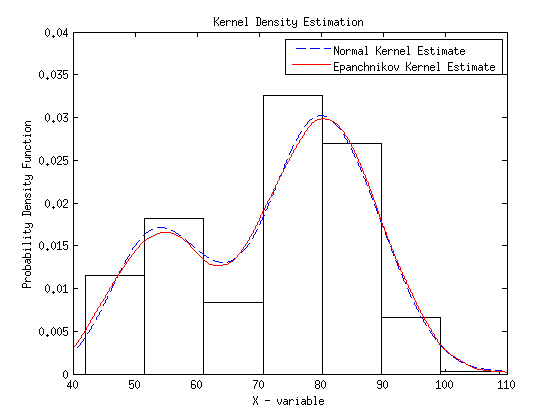
\includegraphics[scale=.86]{inclass_graphb.png}
\caption{Kernel Density Estimation of the Geyser Data Set}
\label{inclass fig2}
\end{center}
\end{figure}
\FloatBarrier

\textbf{Code}

\begin{verbatim}
% use geyser data
load geyser
data = geyser; n = length(data);

% Use Normal Reference Rule for bin width
% of frequency histogram.
h = 2.15*sqrt(var(data))*n^(-1/5);
t0 = min(data)-1;
tm = max(data)+1;
bins = t0:h:tm;
vk = histc(data,bins);
vk(end) = [];
fhat = vk/(n*h);
bc = (t0+h/2):h:(tm-h/2);
bar(bc,fhat,1,'w')
hold on
xlabel('X - variable')
ylabel('Probability Density Function')
title('Kernel Density Estimation')

% Monte Carlos Trials
M = 100;
% choose an appropriate domain
x = linspace(40,110,5000); % domain
% sample size of MC sampling
n = 150;

% find the index for x = x0 = 80
x0ind = find(x>79.999 & x<80.009);    

% NORMAL KERNEL

% choose smoothing parameter
h = 1.06*std(data)*n^(-1/5);

% initialize vector for estimated pdf
fhat = zeros(size(x));

for j = 1:M
    % sample from geyser data
    ind = unidrnd(length(geyser),1,n);
    data = geyser(ind);
    
    % evaluate using the normal kernel for each data point
    % at all x in the domain    
    for i=1:n
        % get each kernel function evaluated at x
        % centered at data and weighted by h
        f=exp(-(1/(2*h^2))*(x-data(i)).^2)/sqrt(2*pi)/h;
        % add each ith average f vector to get estimate pdf height
        fhat = fhat+f/(n);
    end
end
% this is the expected value of fhat based on the MC simulation
fhat = fhat./M;

linenorm = plot(x,fhat,'--b');

% Density estimate using Epanechnikov

% adjust smoothing parameter for the Epanchnikov kernel
h = h*(30*sqrt(pi))^(1/5);

% initialize vector for estimated pdf
fhat = zeros(size(x));

for j = 1:M
    % sample from geyser data
    ind = unidrnd(length(geyser),1,n);
    data = geyser(ind);
    
    % evaluate using the Epanchnikov kernel for each data point
    % at all x in the domain
    for i=1:n
        % set up the indicator function
        I = abs((x-data(i))/h)<1;
        % get each kernel function evaluated at x
        % centered at data
        f=(0.75*(1-(((x-data(i)).^2)/(h^2)))/h).*I;
        fhat = fhat+f/(n);
    end
end

% this is the expected value of fhat based on the MC simulation
fhat = fhat./M;

lineepan = plot(x,fhat,'Color','r');
axis([40 110 0 .04])
legend([linenorm,lineepan],'Normal Kernel Estimate','Epanchnikov Kernel Estimate')
hold off
\end{verbatim}

\clearpage

\section*{Exercise 9.3}
\textbf{Part a.}\\
\textbf{Results \& Discussion: } In this exercise we explore the relationship between the accuracy of the histogram density estimate, as measured by the MSE statistic, and the bin width (smoothing parameter) used. Figure \ref{q3 fig1} below shows that as the number of bins increases (i.e. the smoothing parameter decreases) the MSE seems to increase linearly. This is expected as higher resolution (smaller $h$) leads to higher variability in the estimates.\\

Too large a smoothing parameter makes the estimation meaningless as the density estimate gets closer to being uniform (imagine an estimate with one bin) and increases the estimate's bias. In this particular case it seems that 10 bins would do a reasonable estimation job. In this case the smoothing parameter is $h=0.1414$. 

\begin{figure}[ht!] 
\begin{center}
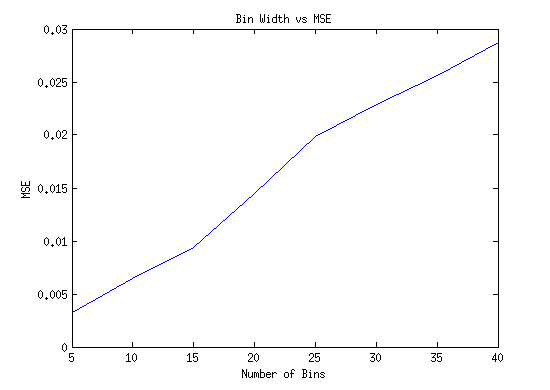
\includegraphics[scale=.86]{q9p3a_graph.png}
\caption{Relationship between bin size and MSE}
\label{q3 fig1}
\end{center}
\end{figure}
\FloatBarrier

\textbf{MSE Results:}
\begin{verbatim}
MSEBIN =

    0.0031    0.0063    0.0107    0.0137    0.0176    0.0227    0.0288    0.0319
\end{verbatim}

\textbf{Code}
\begin{verbatim}
% Monte Carlo trials
M = 1000;
MSE = zeros(1,M);
MSEBIN = [];
for B = 5:5:40
    for i = 1:M;
        n=100;
        x=randn(n,1);
        % Get the histogram-default is 10 bins.
        [vk,bc]=hist(x,B);
        % Get the bin width.
        h = bc(2)-bc(1);
        % Now return an estimate at a point xo.
        xo = 0;
        % Find all of the bin centers less than xo.
        ind = find(bc < xo);
        % xo should be between these two bin centers.
        b1 = bc(ind(end));
        b2 = bc(ind(end)+1);
        % Put it in the closer bin.
        if (xo-b1) < (b2-xo)   % then put it in the 1st bin
            fhat = vk(ind(end))/(n*h);
        else
            fhat = vk(ind(end)+1)/(n*h);
        end
        MSE(i) = (fhat - normpdf(xo))^2;
    end
    MSE  = mean(MSE);
    MSEBIN = [MSEBIN,MSE];
end
plot(MSEBIN)
title('Bin Width vs MSE')
ylabel('MSE')
xlabel('Bin Width')
\end{verbatim}

\textbf{Part b.}\\
\textbf{Results \& Discussion: } In this exercise we explore the relationship between the accuracy of the histogram density estimate, as measured by the MSE statistic, and the sample size. Figure \ref{q3 fig2} below shows that as the sample size gets larger the MSE seems to decrease linearly. This is expected and points to asymptotic consistency of density estimators. The larger the sample size the closer the density estimate will be to the true density. 

\begin{figure}[ht!] 
\begin{center}
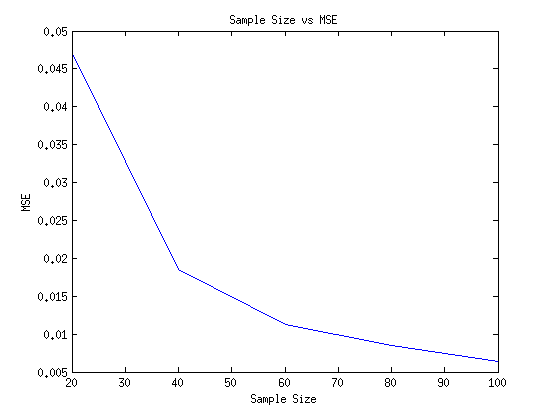
\includegraphics[scale=.86]{q9p3b_graph.png}
\caption{Relationship between sample size and MSE. As the sample size gets larger, the size of the MSE gets smaller.}
\label{q3 fig2}
\end{center}
\end{figure}
\FloatBarrier
\textbf{MSE Results for Increasing Sample Size}
\begin{verbatim}
>> MSESAMP

MSESAMP =

    0.0471    0.0185    0.0113    0.0084    0.0064
\end{verbatim}

\section*{Exercise 9.4}

\textbf{Results \& Discussion}\\
The numbers below are the results for the Monte Carlo trial MSEs of the histogram method, the frequency polygon method and the kernel method of density estimation, in that order. The histogram and the polygon methods show $10^{-3}$ accuracy, while the kernel method shows $10^{-2}$ accuracy. In all three cases it seems the error level is adequate.

\begin{verbatim}
>> MSE = [MSEHIST,MSEFREQ,MSEKER]

MSE =

    0.0009    0.0006    0.0062
\end{verbatim}

\begin{figure}[ht!] 
\begin{center}
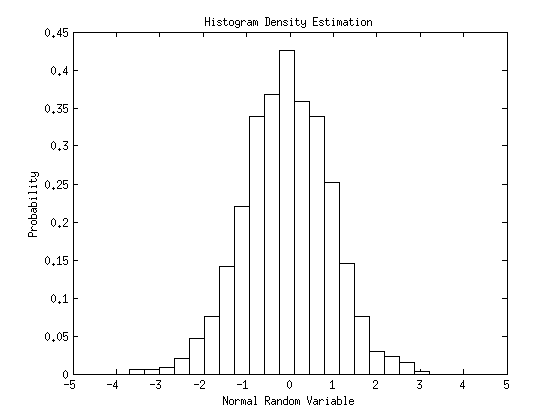
\includegraphics[scale=.86]{q9p4_graph1.png}
\caption{Histogram Method of Density Estimation}
\label{q4 fig1}
\end{center}
\end{figure}
\FloatBarrier

\begin{figure}[ht!] 
\begin{center}
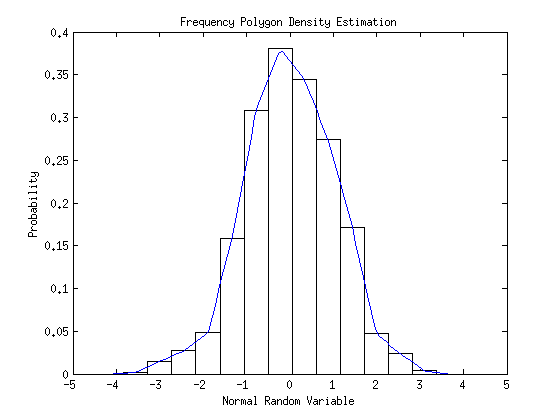
\includegraphics[scale=.86]{q9p4_graph2.png}
\caption{Frequency Polygon Method of Density Estimation}
\label{q4 fig2}
\end{center}
\end{figure}
\FloatBarrier

\begin{figure}[ht!] 
\begin{center}
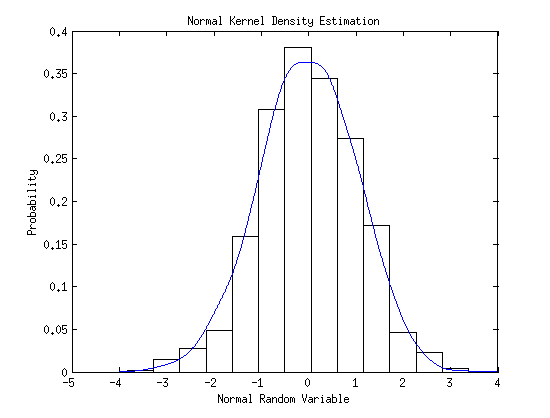
\includegraphics[scale=.86]{q9p4_graph3.png}
\caption{Normal Kernel Method of Density Estimation}
\label{q4 fig3}
\end{center}
\end{figure}
\FloatBarrier

\textbf{Code}
\begin{verbatim}
% sample size
n = 1000;
% monte carlo trials
M = 100;
% value at which to estimate MSE
xo = 0;
MSEHIST = zeros(1,M); MSEFREQ = zeros(1,M); MSEKER = zeros(1,M);

%%%%%%%%%%%%%%%%%%%%%%%%%%%%%%%%%%%%%%%%%%%%%%%%%%%%%%%%%%%%%%%%%%%%%%%%%%%
% HISTOGRAM %
for i = 1:M
    % generate dataset
    data = randn(1,n);
    % Use Normal Reference Rule for bin width.
    h = 3.5*std(data)*n^(-1/3);
    % Get the bin mesh. Put some extra space on the ends.
    t0 = min(data) - 1;
    tm = max(data) + 1;
    rng = tm - t0;
    nbin = ceil(rng/h);
    bins = t0:h:(nbin*h + t0);
    % Get the bin counts vk.
    vk = histc(data,bins);
    
    % Normalize to make it a bona fide density.
    fhathist = vk/(n*h);
    fhathist(end) = [];
    
    % To plot this, use bar with the bin centers.
    tm = max(bins);
    bc = (t0+h/2):h:(tm-h/2);
    
    % calculate MSE
    % Now return an estimate at a point xo.
    % Find all of the bin centers less than xo.
    ind = find(bc < xo);
    % xo should be between these two bin centers.
    b1 = bc(ind(end));
    b2 = bc(ind(end)+1);
    % Put it in the closer bin.
    if (xo-b1) < (b2-xo)   % then put it in the 1st bin
        fhathist0 = vk(ind(end))/(n*h);
    else
        fhathist0 = vk(ind(end)+1)/(n*h);
    end
    MSEHIST(i) = (fhathist0 - normpdf(xo))^2;
end
MSEHIST = mean(MSEHIST);
figure(1)
bar(bc,fhathist,1,'w')
xlabel('Normal Random Variable')
ylabel('Probability')
title('Histogram Density Estimation')

%%%%%%%%%%%%%%%%%%%%%%%%%%%%%%%%%%%%%%%%%%%%%%%%%%%%%%%%%%%%%%%%%%%%%%%%%%%
% FREQUENCY POLYGON %
for i = 1:M
    % generate dataset
    data = randn(1,n);
    % Use Normal Reference Rule for bin width
    % of frequency polygon.
    h = 2.15*sqrt(var(data))*n^(-1/5);
    t0 = min(data)-1;
    tm = max(data)+1;
    bins = t0:h:tm;
    vk = histc(data,bins);
    vk(end) = [];
    fhatfreq = vk/(n*h);
    
    % For freq polygon, get the bin centers, with empty
    % bin center on each end.
    bc2=(t0-h/2):h:(tm+h/2);
    binh = [0 fhatfreq 0];
    % Use linear interpolation between bin centers
    % get the interpolated values at x.
    xinterp = linspace(min(bc2),max(bc2));
    fp = interp1(bc2, binh, xinterp);
    % to plot this, use bar with the bin centers
    tm = max(bins);
    bc = (t0+h/2):h:(tm-h/2);
    
    % calculate MSE
    % Now return an estimate at a point xo.
    % Find all of the bin centers less than xo.
    ind = find(bc < xo);
    % xo should be between these two bin centers.
    b1 = bc(ind(end));
    b2 = bc(ind(end)+1);
    % Put it in the closer bin.
    if (xo-b1) < (b2-xo)   % then put it in the 1st bin
        fhatfreq0 = vk(ind(end))/(n*h);
    else
        fhatfreq0 = vk(ind(end)+1)/(n*h);
    end
    MSEFREQ(i) = (fhatfreq0 - normpdf(xo))^2;
end
MSEFREQ = mean(MSEFREQ);
figure(2)
bar(bc,fhatfreq,1,'w')
hold on
plot(xinterp,fp)
hold off
xlabel('Normal Random Variable')
ylabel('Probability')
title('Frequency Polygon Density Estimation')

%%%%%%%%%%%%%%%%%%%%%%%%%%%%%%%%%%%%%%%%%%%%%%%%%%%%%%%%%%%%%%%%%%%%%%%%%%%
% NORMAL KERNERL %

% choose an appropriate domain
x = linspace(-4,4,1000); % domain

% find the index for x = x0 = 5
x0ind = find(x>-0.999 & x<0.009);

for j = 1:M
    % initialize vector for estimated pdf
    fhatker = zeros(size(x));
    % sample from normal
    data = randn(1,n);
    % choose smoothing parameter
    h = 1.06*std(data)*n^(-1/5);
    
    % evaluate using the normal kernel for each data point
    % at all x in the domain
    for i=1:n
        % get each kernel function evaluated at x
        % centered at data and weighted by h
        f=exp(-(1/(2*h^2))*(x-data(i)).^2)/sqrt(2*pi)/h;
        % add each ith average f vector to get estimate pdf height
        fhatker = fhatker+f/(n);
    end
    % Calculate the expected value of the MSE for x = x0, normal kernel
    MSEKER(j) = mean((normpdf(xo)-fhatker(x0ind)).^2);
end
MSEKER = mean(MSEKER);

figure(3)
bar(bc,fhatfreq,1,'w')
hold on
plot(x,fhatker)
xlabel('Normal Random Variable')
ylabel('Probability')
title('Normal Kernel Density Estimation')
hold off
\end{verbatim}
\clearpage

\section*{Exercise 9.21}

\textbf{Results \& Discussion: } In this exercise we apply two different density estimation methods to the Forearm data. First we use the histogram method applying the Normal Reference Rule to choose the smoothing parameter $h_{hist}=3.5\sigma n^{-\frac{1}{3}}$. Second, we implement the kernel density estimation method using the Normal kernel and the Epanchnikov kernel. Based on these estimates and its graphical representation it appears the data is approximately normal.

\begin{figure}[ht!] 
\begin{center}
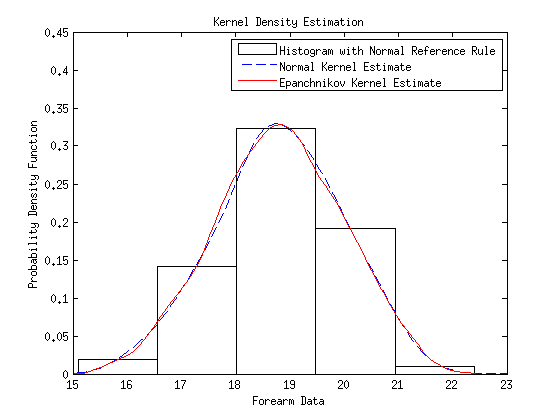
\includegraphics[scale=1]{q9p21_graph1.png}
\caption{Kernel and Histogram methods of density estimation for the forearm data.}
\label{q21 fig1}
\end{center}
\end{figure}
\FloatBarrier

\textbf{Code}
\begin{verbatim}
% use forearm  data
load forearm
data = forearm'; n = length(data);

% Use Normal Reference Rule for bin width
% of frequency histogram.
h = 3.5*sqrt(var(data))*n^(-1/5);
t0 = min(data)-1;
tm = max(data)+1;
bins = t0:h:tm;
vk = histc(data,bins);
vk(end) = [];
fhat = vk/(n*h);
bc = (t0+h/2):h:(tm-h/2);
bar(bc,fhat,1,'w')
hold on
xlabel('Forearm Data')
ylabel('Probability Density Function')
title('Kernel Density Estimation')

% choose an appropriate domain
x = linspace(15,25,100); % domain
% sample size of MC sampling
n = 100;

% NORMAL KERNEL

% choose smoothing parameter
h = 1.06*std(data)*n^(-1/5);

% initialize vector for estimated pdf
fhat = zeros(size(x));

% sample from forearm data
ind = unidrnd(length(forearm),1,n);
data = forearm(ind);

% evaluate using the normal kernel for each data point
% at all x in the domain
for i=1:n
    % get each kernel function evaluated at x
    % centered at data and weighted by h
    f=exp(-(1/(2*h^2))*(x-data(i)).^2)/sqrt(2*pi)/h;
    % add each ith average f vector to get estimate pdf height
    fhat = fhat+f/(n);
end

linenorm = plot(x,fhat,'--b');

% Density estimate using Epanechnikov

% adjust smoothing parameter for the Epanchnikov kernel
h = h*(30*sqrt(pi))^(1/5);

% initialize vector for estimated pdf
fhat = zeros(size(x));

% sample from forearm data
ind = unidrnd(length(forearm),1,n);
data = forearm(ind);

% evaluate using the Epanchnikov kernel for each data point
% at all x in the domain
for i=1:n
    % set up the indicator function
    I = abs((x-data(i))/h)<1;
    % get each kernel function evaluated at x
    % centered at data
    f=(0.75*(1-(((x-data(i)).^2)/(h^2)))/h).*I;
    fhat = fhat+f/(n);
end

lineepan = plot(x,fhat,'Color','r');
axis([15 23 0 .45])
legend('Histogram with Normal Reference Rule','Normal Kernel Estimate','Epanchnikov Kernel Estimate')
hold off
\end{verbatim}
\clearpage

\section*{Exercise 9.22}

\textbf{Results and Discussion:  } In this exercise we explore the heights data and investigate the possibility of finding multiple modes. To do this we increased the resolution of the density estimators by decreasing $h$, the smoothing parameter by a factor of 2 (i.e. we take $h = \frac{h^*}{2}$). We do this for both, the Polygon method and the Kernel method using the Epanchnikov kernel. Figures \ref{q22 fig1} and \ref{q22 fig2} below show the results. It appears that the data may have two modes at approximately $m_1 = 157.5$ and $m_2=162.5$.\\

These possible modes are so close together that they may not be that significant. Also, by decreasing the smoothing parameter, we no longer have an estimation method that minimizes the asymptotic MISE. As shown in exercise 9.3, a finer resolution increases the variability of the estimates and hence the MSE. 


\begin{figure}[ht!] 
\begin{center}
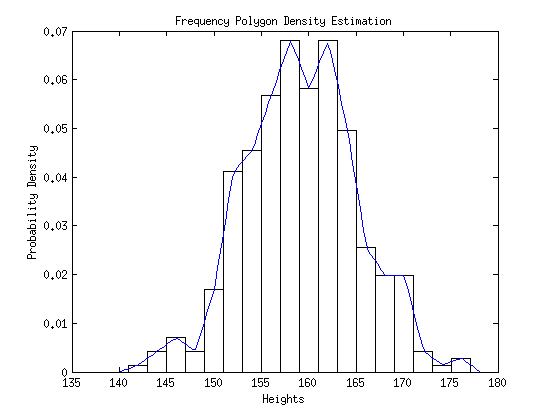
\includegraphics[scale=.86]{q9p22_graph1.png}
\caption{Frequency Polygon method of density estimation for the heights data.}
\label{q22 fig1}
\end{center}
\end{figure}
\FloatBarrier

\begin{figure}[ht!] 
\begin{center}
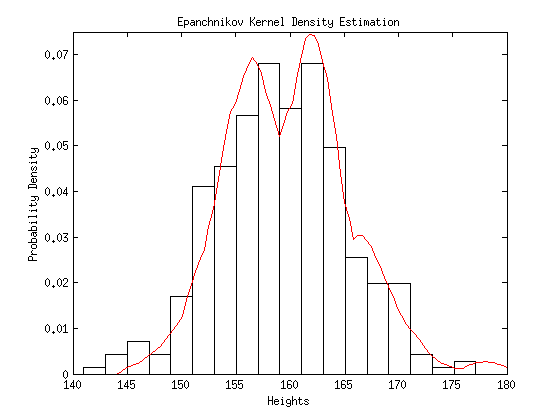
\includegraphics[scale=.86]{q9p22_graph2.png}
\caption{Kernel method of density estimation using the Epanchnikov kernel for the heights data.}
\label{q22 fig2}
\end{center}
\end{figure}
\FloatBarrier

\textbf{Code}
\begin{verbatim}
addpath ~/Documents/Stat572/CompStatsToolboxV2;
% use elderly  data
load elderly
data = heights; n = length(data);

%%%%%%%%%%%%%%%%%%%%%%%%%%%%%%%%%%%%%%%%%%%%%%%%%%%%%%%%%%%%%%%%%%%%%%%%%%%

% FREQUENCY POLYGON %
% Use Normal Reference Rule for bin width
% of frequency polygon.
h = 0.5*2.15*sqrt(var(data))*n^(-1/5);
t0 = min(data)-1;
tm = max(data)+1;
bins = t0:h:tm;
vk = histc(data,bins);
vk(end) = [];
fhatfreq = vk/(n*h);

% For freq polygon, get the bin centers, with empty
% bin center on each end.
bc2=(t0-h/2):h:(tm+h/2);
binh = [0 fhatfreq 0];
% Use linear interpolation between bin centers
% get the interpolated values at x.
xinterp = linspace(min(bc2),max(bc2));
fp = interp1(bc2, binh, xinterp);
% to plot this, use bar with the bin centers
tm = max(bins);
bc = (t0+h/2):h:(tm-h/2);

figure(1)
bar(bc,fhatfreq,1,'w')
hold on
plot(xinterp,fp)
hold off
xlabel('Heights')
ylabel('Probability Density')
title('Frequency Polygon Density Estimation')

%%%%%%%%%%%%%%%%%%%%%%%%%%%%%%%%%%%%%%%%%%%%%%%%%%%%%%%%%%%%%%%%%%%%%%%%%%%
% EPAN KERNERL %

% Use Normal Reference Rule for bin width
% of frequency histogram.
h = 0.5*2.15*sqrt(var(data))*n^(-1/5);
t0 = min(data)-1;
tm = max(data)+1;
bins = t0:h:tm;
vk = histc(data,bins);
vk(end) = [];
fhat = vk/(n*h);
bc = (t0+h/2):h:(tm-h/2);
% plot
figure(2)
bar(bc,fhat,1,'w')
hold on
xlabel('Heights')
ylabel('Probability Density')
title('Epanchnikov Kernel Density Estimation')

% choose an appropriate domain
x = linspace(140,180,100); % domain
% sample size of MC sampling
n = 100;

% Density estimate using Epanechnikov

% adjust smoothing parameter for the Epanchnikov kernel
h = 1.06*std(data)*n^(-1/5);
h = h*(30*sqrt(pi))^(1/5)*.5;

% initialize vector for estimated pdf
fhat = zeros(size(x));

% sample from heights data
ind = unidrnd(length(heights),1,n);
data = heights(ind);

% evaluate using the Epanchnikov kernel for each data point
% at all x in the domain
for i=1:n
    % set up the indicator function
    I = abs((x-data(i))/h)<1;
    % get each kernel function evaluated at x
    % centered at data
    f=(0.75*(1-(((x-data(i)).^2)/(h^2)))/h).*I;
    fhat = fhat+f/(n);
end

% plots
lineepan = plot(x,fhat,'Color','r');
axis([140 180 0 .075])
hold off
\end{verbatim}


\end{document}